\chapter[Giải bài toán hệ thấu kính]{Giải bài toán hệ thấu kính\footnote{Bài đọc thêm}}
\section{Lý thuyết trọng tâm}

\subsection{Hệ hai thấu kính đồng trục ghép cách nhau}
\subsubsection{Sơ đồ tạo ảnh}
Hai thấu kính $L_1$ và $L_2$ có tiêu cự lần lượt là $f_1$ và $f_2$ đặt đồng trục cách nhau một khoảng $a$.
\begin{center}
	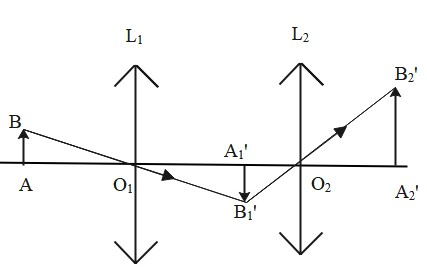
\includegraphics[scale=0.8]{../figs/VN11-PH-39-L-027-1-h28.jpg}
\end{center}

Vật AB có ảnh $\text{A'}_1\text{B}'_1$ tạo bởi thấu kính $L_1$. $\text{A'}_1\text{B}'_1$ lại là vật đối với thấu kính $L_2$, cho ảnh $\text{A'}_2\text{B}'_2$ tạo bởi thấu kính $L_2$.

Toàn bộ quá trình tạo ảnh được tóm tắt sơ đồ tạo ảnh:
\begin{equation}
{AB}\xrightarrow[d_1;\ d'_1]{L_1} \text{A}'_1\text{B}'_1 \xrightarrow[d_2;\ d'_2]{L_2}\text{A}'_2\text{B}'_2
\end{equation}
	
Với: 
\begin{itemize}
	\item $d_1,\ d'_1$ là khoảng từ từ AB và $\text{A'}_1\text{B}'_1$ đến thấu kính $L_1$;
	\item $d_2,\ d'_2$ là khoảng từ từ $\text{A'}_1\text{B}'_1$ và $\text{A'}_2\text{B}'_2$ đến thấu kính $L_2$.
\end{itemize}




\subsubsection{Vị trí, tính chất của ảnh tạo bởi hệ thấu kính}
\begin{center}
	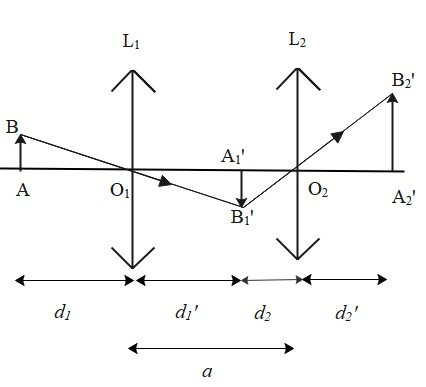
\includegraphics[scale=0.8]{../figs/VN11-PH-39-L-027-1-h29.jpg}
\end{center}

Đối với thấu kính $L_1$:
$$d_1=\overline{\text{O}_1\text{A}};\quad d'_1=\overline{\text{O}_1\text{A}'_1}=\dfrac{f_1\cdot d_1}{d_1-f_1}.$$

Đối với thấu kính $L_2$:
$$d_2=\overline{\text{O}_2\text{A}'_1}=a-d'_1;\quad d'_2=\overline{\text{O}_2\text{A}'_2}=\dfrac{f_2\cdot d_2}{d_2-f_2}.$$

Nếu:
\begin{itemize}
	\item $d'_2>0\Rightarrow$ ảnh $\text{A}'_2\text{B}'_2$ là ảnh thật. 
	\item $d'_2<0\Rightarrow$ ảnh $\text{A}'_2\text{B}'_2$ là ảnh ảo.
\end{itemize}

Độ phóng đại của ảnh qua hệ thấu kính:
$$k=\dfrac{\overline{\text{A}'_2\text{B}'_2}}{\overline{\text{AB}}}=\dfrac{\overline{\text{A}'_2\text{B}'_2}}{\overline{\text{A}'_1\text{B}'_1}}\cdot  \dfrac{\overline{\text{A}'_1\text{B}'_1}}{\overline{\text{AB}}}=k_2\cdot k_1.$$

Nếu:
\begin{itemize}
	\item $k>0\Rightarrow$ ảnh $\text{A}'_2\text{B}'_2$ cùng chiều với vật AB. 
	\item $k<0\Rightarrow$ ảnh $\text{A}'_2\text{B}'_2$ ngược chiều với vật AB.
\end{itemize}

Độ cao của ảnh qua hệ thấu kính: $$\text{A}'_2\text{B}'_2=|k|\cdot AB.$$
\subsection{Hệ hai thấu kính đồng trục ghép sát nhau}
\subsubsection{Sơ đồ tạo ảnh}
Hai thấu kính $L_1$ và $L_2$ có tiêu cự lần lượt là $f_1$ và $f_2$ được ghép sát nhau $(a=0)$.
\begin{center}
	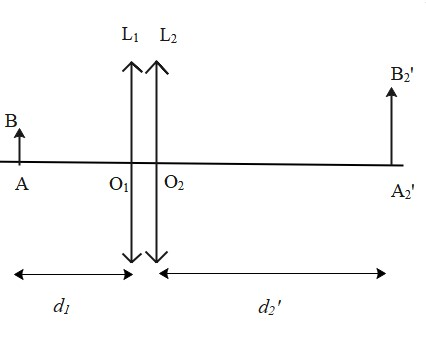
\includegraphics[scale=0.8]{../figs/VN11-PH-39-L-027-1-h30.jpg}
\end{center}
Sơ đồ tạo ảnh:
\begin{equation}
\text{AB}\xrightarrow[d_1;\ d'_2]{L} \text{A}'_2\text{B}'_2 
\end{equation}

Hai thấu kính tương đương với một thấu kính duy nhất có độ tụ và tiêu cự như sau: 
\begin{equation}
D = D_1 +D_2\qquad  \text{và}\qquad  \dfrac{1}{f}=\dfrac{1}{f_1}+\dfrac{1}{f_2},
\end{equation}
với $D_1,\ D_2$ lần lượt là độ tụ của thấu kính $L_1,L_2$.

\subsubsection{Vị trí, tính chất của ảnh tạo bởi hệ thấu kính}

Đặc điểm ảnh của vật AB tạo bởi hệ hai thấu kính ghép là đặc điểm ảnh của vật AB tạo bởi thấu kính tuương đương. Ta cũng sử dựng các công thức như hệ thấu kính cách nhau một khoảng $a$ nhưng lúc này $a=0$.


\section{Bài tập }
\begin{dang}{Hệ hai thấu kính đồng trục ghép cách nhau}
\end{dang}
\textbf{Phương pháp giải}
\begin{description}
	\item[Bước 1:] Lập sơ đồ tạo ảnh của hệ thấu kính.
	\item[Bước 2:] Áp dụng các công thức thấu kính lần lượt cho mỗi thấu kính.

	$ d'_1=\dfrac{f_1\cdot d_1}{d_1-f_1};\quad d_2=a-d'_1;\quad d'_2=\dfrac{f_2\cdot d_2}{d_2-f_2};\quad k=k_1\cdot k_2$.
	\item[Bước 3:] Xác định vị trí, tính chất, độ cao của ảnh tạo bởi hệ thấu kính.
\end{description}
\vspace{1em}
\viduii{3}{
Cho một hệ gôm hai thấu kính hội tụ $L_1$ và $L_2$ có tiêu cự lần lượt là $f_1=30\ \text{cm}$ và $f_2=20\ \text{cm}$ đặt đồng trục cách nhau $a=60\ \text{cm}$. Vật sáng AB cao 3 cm đặt vuông góc với trục chính (A ở trên trục chính) trước thấu kính $L_1$ cách $O_1$ một khoảng $d_1=45\ \text{cm}$. Hãy xác định vị trí, tính chất, độ cao của ảnh cuối cùng $\text{A}'_2\text{B}'_2$ qua hệ thấu kính trên.
\begin{mcq}
	\item Ảnh $\text{A}'_2\text{B}'_2$ là ảnh ảo, cách thấu kính $L_2$ là 12 cm, ngược chiều vật AB và có độ cao bằng $\text{2,4}\ \text{cm}$.
	\item Ảnh $\text{A}'_2\text{B}'_2$ là ảnh thật, cách thấu kính $L_2$ là 12 cm, ngược chiều vật AB và có độ cao bằng $\text{2,4}\ \text{cm}$.
	\item Ảnh $\text{A}'_2\text{B}'_2$ là ảnh thật, cách thấu kính $L_2$ là 24 cm, ngược chiều vật AB và có độ cao bằng $\text{2,4}\ \text{cm}$.
	\item Ảnh $\text{A}'_2\text{B}'_2$ là ảnh ảo, cách thấu kính $L_2$ là 24 cm, ngược chiều vật AB và có độ cao bằng $\text{2,4}\ \text{cm}$.
\end{mcq}}{
\begin{center}
	\textbf{Hướng dẫn giải:}
\end{center}

{ Sơ đồ tạo ảnh:
	
	${AB}\xrightarrow[d_1;\ d'_1]{L_1} \text{A}'_1\text{B}'_1 \xrightarrow[d_2;\ d'_2]{L_2}\text{A}'_2\text{B}'_2$
	
	Đối với ảnh $\text{A}'_1\text{B}'_1$ tạo bởi thấu kính $L_1$: 
	$\begin{cases} d_1=45\ \text{cm} \\ d'_1=\dfrac{d_1\cdot f_1}{d_1-f_1}=90\ \text{cm}\end{cases}$
	
	Đối với ảnh $\text{A}'_2\text{B}'_2$ tạo bởi thấu kính $L_2$: 
	$\begin{cases} d_2=a-d'_1=60-90=-30\ \text{cm} \\ d'_2=\dfrac{d_2\cdot f_2}{d_2-f_2}=12\ \text{cm}>0\ (1)\end{cases}$
	
	Số phóng đại của ảnh qua hệ thấu kính:
	
	$k=\dfrac{\overline{\text{A}'_2\text{B}'_2}}{\overline{\text{A}'_1\text{B}'_1}}\cdot \dfrac{\overline{\text{A}'_1\text{B}'_1}}{\overline{\text{AB}}}=\dfrac{d'_1}{d_1}\cdot \dfrac{d'_2}{d_2}=-\dfrac{4}{5}<0\ (2)$.
	
	Độ cao của ảnh $\text{A}'_2\text{B}'_2$ qua hệ thấu kính:
	 $\text{A}'_2\text{B}'_2=|k|\cdot \text{AB}=\text{2,4}\ \text{cm}\ (3)$.
	 
	Từ $(1), \ (2), \ (3)$ suy ra ảnh cuối cùng $\text{A}'_2\text{B}'_2$ là ảnh thật, cách thấu kính $L_2$ một đoạn 12 cm, ngược chiều với vật AB và có độ cao bằng $\text{2,4}\ \text{cm}$.
	
\textbf{	Đáp án: B.}
}
}
\viduii{3}{
Một vật sáng AB cao 1 cm được đặt vuông góc trục chính của một hệ gồm hai thấu kinh $L_1$ và $L_2$ đồng trục cách thấu kính $L_1$ một khoảng $d_2=30\ \text{cm}$.Thấu kính $L_1$ là thấu kính hội tụ có tiêu cự  
$f_1=20\ \text{cm}$, thấu kính $L_2$ là thấu kính phân kỳ có tiêu cự $f_2=-30\ \text{cm}$, hai thấu kính cách nhau $a=40\ \text{cm}$. Hãy xác định vị trí, tính chất, độ cao của ảnh cuối cùng $\text{A}'_2\text{B}'_2$ qua hệ thấu kính trên.
\begin{mcq}
	\item Ảnh $\text{A}'_2\text{B}'_2$ là ảnh thật, cách thấu kính $L_2$ là 30 cm, ngược chiều vật AB và có độ cao bằng $\text{6}\ \text{cm}$.
	\item Ảnh $\text{A}'_2\text{B}'_2$ là ảnh ảo, cách thấu kính $L_2$ là 60 cm, cùng chiều vật AB và có độ cao bằng $\text{6}\ \text{cm}$.
	\item Ảnh $\text{A}'_2\text{B}'_2$ là ảnh ảo, cách thấu kính $L_2$ là 60 cm, ngược chiều vật AB và có độ cao bằng $\text{6}\ \text{cm}$.
	\item Ảnh $\text{A}'_2\text{B}'_2$ là ảnh thật, cách thấu kính $L_2$ là 60 cm, ngược chiều vật AB và có độ cao bằng $\text{6}\ \text{cm}$.
\end{mcq}}{
\begin{center}
	\textbf{Hướng dẫn giải:}
\end{center}

{ Sơ đồ tạo ảnh:
	
	${AB}\xrightarrow[d_1;\ d'_1]{L_1} \text{A}'_1\text{B}'_1 \xrightarrow[d_2;\ d'_2]{L_2}\text{A}'_2\text{B}'_2$
	
	Đối với ảnh $\text{A}'_1\text{B}'_1$ tạo bởi thấu kính $L_1$: 
	$\begin{cases} d_1=30\ \text{cm} \\ d'_1=\dfrac{d_1\cdot f_1}{d_1-f_1}=60\ \text{cm}\end{cases}$
	
	Đối với ảnh $\text{A}'_2\text{B}'_2$ tạo bởi thấu kính $L_2$: 
	$\begin{cases} d_2=a-d'_1=40-60=-20\ \text{cm} \\ d'_2=\dfrac{d_2\cdot f_2}{d_2-f_2}=60\ \text{cm}>0\ (1)\end{cases}$
	
	Số phóng đại của ảnh qua hệ thấu kính:
	
	$k=\dfrac{\overline{\text{A}'_2\text{B}'_2}}{\overline{\text{A}'_1\text{B}'_1}}\cdot \dfrac{\overline{\text{A}'_1\text{B}'_1}}{\overline{\text{AB}}}=\dfrac{d'_1}{d_1}\cdot \dfrac{d'_2}{d_2}=-6<0\ (2)$.
	
	Độ cao của ảnh $\text{A}'_2\text{B}'_2$ qua hệ thấu kính:
	$\text{A}'_2\text{B}'_2=|k|\cdot \text{AB}=\text{6}\ \text{cm}\ (3)$.
	
	Từ $(1), \ (2), \ (3)$ suy ra ảnh cuối cùng $\text{A}'_2\text{B}'_2$ là ảnh thật, cách thấu kính $L_2$ một đoạn 60 cm, ngược chiều với vật AB và có độ cao bằng $\text{6}\ \text{cm}$.
	
	
	
\textbf{	Đáp án: B.}
}}

\begin{dang}{Hệ hai thấu kính đồng trục ghép sát nhau}
\end{dang}
\textbf{Phương pháp giải}
\begin{description}
	\item[Bước 1:] Lập sơ đồ tạo ảnh của hệ thấu kính.
	\item[Bước 2:] Áp dụng các công thức thấu kính lần lượt cho mỗi thấu kính.
	
	$D = D_1 +D_2\  \text{và}\  \dfrac{1}{f}=\dfrac{1}{f_1}+\dfrac{1}{f_2}.$
		\item[Bước 3:] Xác định vị trí, tính chất, độ cao của ảnh tạo bởi hệ thấu kính.
\end{description}
\vspace{1em}
\vidu{3}{
Một thấu kính phân kỳ có tiêu cự $f_1=-20\ \text{cm}$. Thấu kính được đặt sao cho trục chính thẳng đứng, mặt lõm hướng lên trên.
\begin{center}
	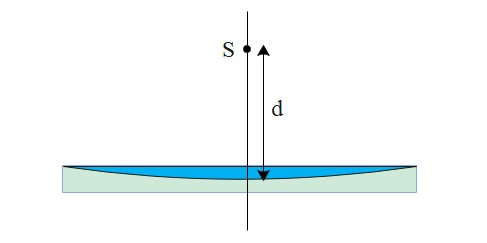
\includegraphics[scale=0.8]{../figs/VN11-PH-39-L-027-1-h31.jpg}
\end{center}
\begin{enumerate}
	\item Ảnh S' của S tạo bởi thấu kính cách thấu kính 12cm. Tính khoảng cách $d$ từ S đến thấu kính.
	\item Giữ S và thấu kính cố định. Đổ một lớp chất lỏng trong suốt vào mặt lõm. Bây giờ ảnh S' của S cách thấu kính 20 cm. Tính tiêu cự $f_2$ của lớp chất lỏng làm thấu kính.
	
\end{enumerate}	
}
{

\begin{center}
	\textbf{Hướng dẫn giải:}
\end{center}

{\begin{enumerate}
	\item S có ảnh tạo bởi thấu kính phân kỳ: $d'_1=-12\ \text{cm}$.
	
	Do đó: 
	$\dfrac{1}{f_1}=\dfrac{1}{d_1}+\dfrac{1}{d'_1}\Rightarrow \dfrac{1}{d_1}=\dfrac{1}{f_1}-\dfrac{1}{d'_1}=\dfrac{1}{30}$.
	
	Suy ra: $d=30\ \text{cm}$.
	\item Hệ gồm thấu kính chất lỏng và thấu kính thủy tinh ghép đồng trục, sát nhau.
	
	Thấu kính tương đương có tiêu cự $f$.
	Ta có sơ đồ tạo ảnh:
	\begin{equation}
	\text{S}\xrightarrow[d;\ d']{L} \text{S'}
	\end{equation}
		
	Ta có: $\dfrac{1}{f}=\dfrac{1}{f_1}+\dfrac{1}{f_2}$.
	
	Đối với thấu kính tương đương: $d'=-20\ \text{cm}$.
	
	Vậy: $\dfrac{1}{f}=\dfrac{1}{d}+\dfrac{1}{d'}=-\dfrac{1}{60}$.
	
	Suy ra: $\dfrac{1}{f_2}=\dfrac{1}{f}-\dfrac{1}{f_1}=\dfrac{1}{30}$.
	
	Vậy tiêu cự $f_2$ của lớp chất lỏng làm thấu kính là $30\ \text{cm}$.
	
\end{enumerate}
		

	\textbf{Đáp án: B.}
}
}